%
% This is the LaTeX template file for lecture notes for CS294-8,
% Computational Biology for Computer Scientists.  When preparing 
% LaTeX notes for this class, please use this template.
%
% To familiarize yourself with this template, the body contains
% some examples of its use.  Look them over.  Then you can
% run LaTeX on this file.  After you have LaTeXed this file then
% you can look over the result either by printing it out with
% dvips or using xdvi.
%
% This template is based on the template for Prof. Sinclair's CS 270.

\documentclass[11pt, twosides]{article}
\usepackage[utf8]{inputenc}
\usepackage{graphicx}
\usepackage{hyperref}
\usepackage{graphics}
\usepackage{amsmath}
\usepackage{amsfonts}
\usepackage{amssymb}
\usepackage{amsthm}
\usepackage{xcolor}
\setlength{\oddsidemargin}{0.25 in}
\setlength{\evensidemargin}{-0.25 in}
\setlength{\topmargin}{-0.6 in}
\setlength{\textwidth}{6.5 in}
\setlength{\textheight}{8.5 in}
\setlength{\headsep}{0.75 in}
\setlength{\parindent}{0 in}
\setlength{\parskip}{0.1 in}

%
% The following commands set up the lecnum (lecture number)
% counter and make various numbering schemes work relative
% to the lecture number.
%
\newcounter{lecnum}
\renewcommand{\thepage}{\thelecnum-\arabic{page}}
\renewcommand{\thesection}{\thelecnum.\arabic{section}}
\renewcommand{\theequation}{\thelecnum.\arabic{equation}}
\renewcommand{\thefigure}{\thelecnum.\arabic{figure}}
\renewcommand{\thetable}{\thelecnum.\arabic{table}}

%
% The following macro is used to generate the header.
%
\newcommand{\lecture}[4]{
%   \pagestyle{myheadings}
   \thispagestyle{plain}
   \newpage
   \setcounter{lecnum}{#1}
   \setcounter{page}{1}
   \noindent
   \begin{center}
   \framebox{
      \vbox{\vspace{2mm}
    \hbox to 6.28in { {\bf CS 419M Introduction to Machine Learning
                        \hfill Spring 2021-22} }
       \vspace{4mm}
       \hbox to 6.28in { {\Large \hfill Lecture #1: #2  \hfill} }
       \vspace{2mm}
       \hbox to 6.28in { {\it Lecturer: #3 \hfill Scribe: #4} }
      \vspace{2mm}}
   }
   \end{center}
   \markboth{Lecture #1: #2}{Lecture #1: #2}
}

%
% Convention for citations is authors' initials followed by the year.
% For example, to cite a paper by Leighton and Maggs you would type
% \cite{LM89}, and to cite a paper by Strassen you would type \cite{S69}.
% (To avoid bibliography problems, for now we redefine the \cite command.)
% Also commands that create a suitable format for the reference list.
% \renewcommand{\cite}[1]{[#1]}
% \def\beginrefs{\begin{list}%
%         {[\arabic{equation}]}{\usecounter{equation}
%          \setlength{\leftmargin}{2.0truecm}\setlength{\labelsep}{0.4truecm}%
%          \setlength{\labelwidth}{1.6truecm}}}
% \def\endrefs{\end{list}}
% \def\bibentry#1{\item[\hbox{[#1]}]}

%Use this command for a figure; it puts a figure in wherever you want it.
%usage: \fig{NUMBER}{SPACE-IN-INCHES}{CAPTION}
% \newcommand{\fig}[3]{
% 			\vspace{#2}
% 			\begin{center}
% 			Figure \thelecnum.#1:~#3
% 			\end{center}
% 	}
% Use these for theorems, lemmas, proofs, etc.
\newtheorem{theorem}{Theorem}[lecnum]
\newtheorem{lemma}[theorem]{Lemma}
\newtheorem{proposition}[theorem]{Proposition}
\newtheorem{claim}[theorem]{Claim}
\newtheorem{corollary}[theorem]{Corollary}
\newtheorem{definition}[theorem]{Definition}
%\newenvironment{proof}{{\bf Proof:}}{\hfill\rule{2mm}{2mm}}

% **** IF YOU WANT TO DEFINE ADDITIONAL MACROS FOR YOURSELF, PUT THEM HERE:

\begin{document}
%FILL IN THE RIGHT INFO.
%\lecture{**LECTURE-NUMBER**}{**DATE**}{**LECTURER**}{**SCRIBE**}
\lecture{11}{Some Problems}{Abir De}{Group 11}
%\lecture{x}{Title}{Abir De}{Group y}
\section{Regularization of bias}
The primary aim of adding a bias in our model is to have clearly demarcated decision boundaries.Theoretically, the bias can be regularized, but in practice it makes little sense to do the same. For the purpose of regularization, the bias can be taken as a hyperparameter along with w i.e.,
\begin{equation*}
    [w,b]\cdot[x,1] = w^Tx+b
\end{equation*}
But rather than adding separate term of $\lambda b^2$ to our loss function, the performance of the model can instead be analyzed by using cross validation.\\
Moreover, there might be cases where w is small but the corresponding bias is high.
Consider the following scenario shown in figure - 
\newline
\begin{figure}[h]
    \centering
    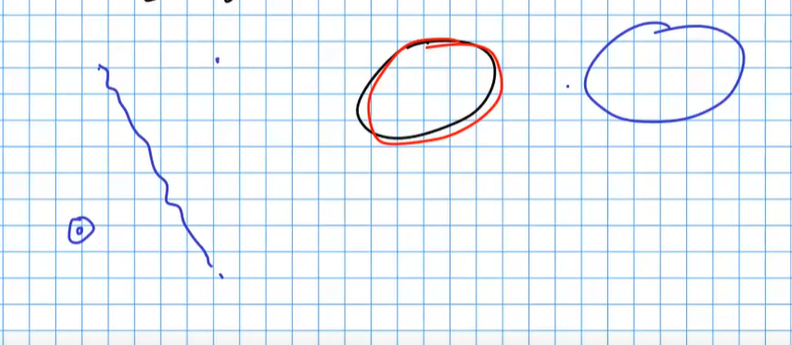
\includegraphics[scale = 0.5]{pictures/ifbregularise.png}
    \caption{If the bias is regularized}
\end{figure}


Here, unless the origin isn't between the two clusters shown, regularization of the bias has no added advantage for the model. Therefore, regularization of bias generally leads to underfitting and is usually not the method adopted.


\newpage 

\section{Stability of Ranking Loss}
We have the ranking loss for all pairs of $x_{bad}$ and $x_{good}$ given by -
$${f(w) = \sum_{\substack{y_{bad}=-1 \\ y_{good}=+1 \\ x_{bad,good}\in S}}( 1 + w^{T}x_{bad} -  w^{T}x_{good})}$$

What should be the regularizer $\lambda$ that should be added to the loss to ensure that it is stable?

Suggestion - If we consider $x_{bad} - x_{good}$ as a new proxy variable , then the regulariser will be the number of pairs of $x_{bad}$ and $x_{good}$. So the loss function becomes
$${f(w) = \sum_{\substack{y_{bad}=-1 \\ y_{good}=+1 \\ x_{bad,good}\in S}}( 1 + w^{T}x_{bad} -  w^{T}x_{good}) + \lambda |S_{good}||S_{bad}|||w||^2}$$

However proving the stability for this is not the same as proving the stability for a single variable as before because here, when we change the set S by replacing an old point with a new point ${x,y}$ to get $S^{'}$, all pairs in the summation of which it is a part will change. Thus, this is different from a point-wise loss. 

Optimal w can be easily found for this case by differentiating the loss term wrt w to get

$${w = \sum\frac{(x_{good} - x_{bad})}{2\lambda|S_{good}||S_{bad}|}}$$

What would it be if the loss was calculated using the hinge function and what is the condition of stability?
$${f(w) = \sum_{\substack{y_{bad}=-1 \\ y_{good}=+1 \\ x_{bad,good}\in S}}( 1 + w^{T}x_{bad} -  w^{T}x_{good})_{+} + \lambda |S_{good}||S_{bad}|||w||^2}$$

Following the same line of proof as earlier, we will get some bound in terms of ${\frac{1}{|S_{good}|} or \frac{1}{|S_{bad}|}}$

But can we find some regulariser that is independent of the ratio of $x_{good}$ to $x_{bad}$?

Solution - If we use the following regulariser, though we would be over-regularising w but we can be ensured stability.

$${\frac {|S|(|S|-1)}{2}}$$
\newpage 
\section{Formation of Dual}
Say we are dealing with the traditional linear regression problem. That is, given a dataset $\mathfrak{D}$,
\[\mathfrak{D} = \{(x_i,y_i) \mid i \in [|\mathfrak{D}|], x_i \in \mathbb{R}^d, y_i \in \mathbb{R}\}\]
where, $[n] := \{1,2, \dots n\} \forall n \in \mathbb{N}$.


We want to perform the following minimization,
\[\underset{{w}}{\text{min}}\sum_{i}(y_i - {w}^Tx_i)^2 + ||w||^2\]
We ask the following question.
\begin{center}
    \underline{Question} Can we obtain the dual form of this problem, just like we did in the case of classification?
\end{center}
We will start by converting this unconstrained optimization to a constrained optimization problem. Further, we should check whether the constrained optimization problem is convex.
With the idea of minimizing each of the square terms in mind, we define $\zeta_i$ such that
\[\zeta_i \geq (y_i - w^Tx_i) \text{ ,with } \zeta_i \geq 0 \text{ } \forall i\]
Thus now we have the problem:
\[\underset{w,\zeta_i}{min}(\sum_i\zeta_i + \lambda||w||^2)\]
\[\textit{such that } \zeta_i \geq (y_i - w^Tx_i) \text{ } \forall i\]
Now, the second equation above gives us the constraint, and then we have
\[\underset{\alpha_i,\beta_i}{max}\text{ }\underset{w,\zeta_i}{min}\left(\lambda||w||^2 + \sum_i(\zeta_i + \alpha((y_i - w^Tx_i)^2 - \zeta_i) - \beta_i\zeta_i)\right)\]
Further note that at the optimum value of $\zeta_i = \zeta_i^*$, the following would hold,
\[(y_i - w^Tx_i)^2 = \zeta_i^* \text{ } \forall i \text{   (Why?)}\]

\newpage 
\section{Dimension of $\mathbf{w}$}
Suppose we are given a data set $\mathfrak{D}$,
\[\mathfrak{D} = \{(x_i,y_i) \mid i \in [|\mathfrak{D}|], x_i \in \mathbb{R}, y_i \in \mathbb{R}\}\]
where, $[n] := \{1,2, \dots n\} \forall n \in \mathbb{N}$. Denote,
\[\mathfrak{D}\mid_x := \{x_i \mid (x_i,y_i) \in \mathfrak{D}\}\]
\[\mathfrak{D}\mid_y := \{y_i \mid (x_i,y_i) \in \mathfrak{D}\}\]
\\ 
Further suppose that the data set is distributed around some line given by $y = mx + c$.
That is, \[y_i = mx_i + c + \epsilon_i \text{ } \forall i \in [|\mathfrak{D}|]\]
where $\epsilon_i \sim \mathbb{P}(\cdot)$. Thus we have the following picture,
\begin{figure}[h]
    \centering
    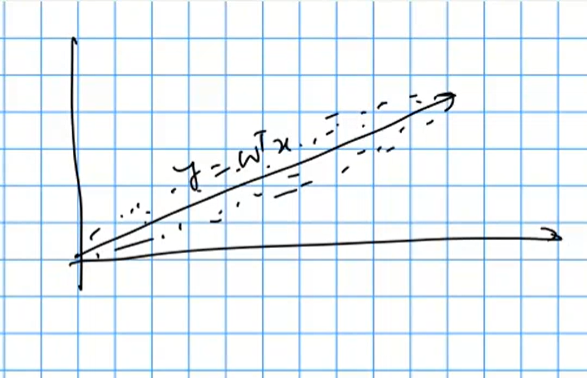
\includegraphics[height = 5cm, width = 5cm]{pictures/q4.PNG}
    \caption{A picture of the data}
\end{figure}


Now, for each $x_i \in \mathfrak{D}\mid_x$, and for all $n \in \mathbb{N}$, define,
\[\mathbf{x}_i := (x_i,x_i^2 \dots x_i^n)^T \in \mathbb{R}^n\]
Further, let $\mathbf{w} \in \mathbb{R}^n$. We ask the following question,
\begin{center}
    \underline{Question} What is the $n$, such that we can be \textit{assured} that the following holds: 
    \[y_i = \mathbf{w}^T\mathbf{x}_i \forall y_i \in \mathfrak{D}_y\]
\end{center}
Informally, in the extreme overfitting case, what is the minimum error that we get -- and what is the corresponding dimension of the weights vector, that is $n$?

Note the following lemma.
\begin{lemma}
Given $n+1$ points $(x_i,y_i)$ with $n \geq 1$, such that all the $x_i$ are distinct. There exists a $n$ degree polynomial $p$ with coefficients $(a_n,a_{n-1}, \dots a_0)$ such that
\[p(x_i) = y_i \forall i \in [n+1]\]
\end{lemma}
\begin{proof}
We have the following equations,
\[a_nx_i^n + a_{n-1}x_i^{n-1} + \dots a_0 = y_i \forall i \in [n+1]\]
This can be expressed in the matrix form as,
\[\begin{pmatrix} x_1^n & x_1^{n-1} & \dots &x_1& 1 \\ 
\vdots & \vdots & \ddots &\vdots&\vdots \\  x_{n+1}^n & x_{n+1}^{n-1} & \dots &x_{n+1}& 1
\end{pmatrix} \begin{pmatrix} a_n \\ a_{n-1} \\ \vdots \\ a_0 \end{pmatrix} = \begin{pmatrix}y_{0} \\ y_1 \\ \vdots \\ y_{n+1}\end{pmatrix}
\]
Note that the matrix on the left is a Vandermonde matrix, and has a non zero determinant. Thus the system of equations has a unique solution.
\end{proof}


For our case, since we do not have a bias term (note the definition of $\mathbf{x}_i$), our equations would be of the form,
\[a_nx_i^n + a_{n-1}x_i^{n-1} + \dots + a_1x_i = y_i\]
Thus (assume non zero $x_i$), 
\[a_nx_i^{n-1} + a_{n-1}x^{n-2} + \dots + a_1 = y_i/x_i\]
By the previous lemma, we have,
\[n - 1 = |\mathfrak{D}| - 1\]
Thus, \[n = |\mathfrak{D}|\]
Thus, we should have,
\[\text{dim}(\mathbf{w}) \leq |\mathfrak{D}|\]
\hfill\qedsymbol


But, this says that the number of parameters is dependent on the number of features! This should not be the case! \\ 
Interestingly, in deep learning, networks are more often than not extremely overparametrised (look up some typical neural nets) - and still we obtain good generalization errors! So, even with a \textit{lot} of parameters \textit{without} regularization, the deep learning model will ``understand" the situation and put certain weights to zero!



\section{Group Details and Individual Contribution}

\begin{center}
\begin{tabular}{|c | c| }
\hline 
Problem  & Scribe\\ \hline
Regularization of Bias  & Raavi Gupta (200070064)\\ \hline
Stability of Ranking Loss  & Latika Patel (180100062)\\ \hline
Formation of Dual  & Siddhant Midha (200070078)\\ \hline
Dimension of $\mathbf{w}$   & Siddhant Midha (200070078)\\ \hline
\end{tabular}
\end{center}
\end{document}





